\chapter{Implementation}
\label{chapter:implementation}

\begin{itemize}
  \item intro
  \item Vi lager en liten prototype = ``proof of concept'' -> et begrep vi m\aa~bruke =)
  \item VarRefs m\aa~sendes oppover fra child nodes (ref til tainting deps)
  \item Optimalisering: child nodes vet om de er atomiske/singleton eller ikke
\end{itemize}

\begin{itemize}
  \item Bruk av parseren (den som er generert av antlr osv), XQFTTree-klassen,
  evt. UML
  \item Interfacing av parseren mot oversetteren v\aa r (som oversetter til
  relalg) og UML
  \item Bygging av relasjonsalgebra-tre, UML av operatorklassene
  \item Implementering av visitors
  \item Scoping og symtab (nok en gang..)
  \item hvordan metadata som varrefs og singletonindikering blir sendt oppover
  (Metadata)
  \item Implementering av ``tainting dependencies''
  \item Dataflyt ()
  \item Visible external API
  \item Interface til systemet p\aa~ kommandolinjen
  \item Optimaliseringer, om noen? 
\end{itemize}

\section{Prerequisites}
This proof of concept was implemented in Java 5.0, using regular object
oriented techniques, and is licensed under a liberal BSD license. Instructions
for compilation and installation can be found in TODO: appendix.

\section{Using the XQFT Parser}
The \textit{XQFT Parser}\cite{ourselves} (described in section
\ref{sect:theory:xqftparser}) is a prerequisite for providing the abstract
syntax tree for this XQuery translator. This section will outline how this
parser was used and interfaced with the implementation.

\subsection{Basics and API}
The \textit{XQFT Parser} is a parser generated by the ANTLR parser generator.
Thus, there is a loosely standardised API available for any implementor
utilising a parser generated by ANTLR. In the case of \textit{XQFT Parser}, two
classes are generated: \texttt{XQFTParser} and \texttt{XQFTLexer}. These
classes are used in conjunction on an input string to produce an abstract syntax
tree (see next subsection, and also section
\ref{sect:theory:xqftparser:ast_construction}).

A typical use case to achieve this is shown in figure \ref{}

\begin{figure}[!htp]
\begin{center}
  \begin{Verbatim}
    CharStream cs 
        = new ANTLRStringStream(
            "for $i in (1,2,3) return $i");

    XQFTLexer lexer = new XQFTLexer(cs);

    UnbufferedCommonTokenStream tokens 
        = new UnbufferedCommonTokenStream();
	tokens.setTokenSource(lexer);

    XQFTParser parser = new XQFTParser(tokens);
    parser.setTreeAdaptor(new XQFTTreeAdaptor());
    parser.setLexer(lexer);

    XQFTTree ast = parser.module().getTree();
  \end{Verbatim}
  \caption{Using the XQFTParser and XQFTLexer classes}
  \label{figure:impl:using_xqft}
\end{center}
\end{figure}

\subsection{The XQFTTree class}
\subsection{Interfacing the XQFT Parser}
\section{Constructing the MQL algebra tree}
\label{sect:impl:construct_mql}
The MQL queries are constructed as a tree of operators bottom-up while parsing
the abstract syntax tree (for the corresponding XQuery query). 

\subsection{Operators and parameters}
\begin{figure}[!htp]
\begin{center}
  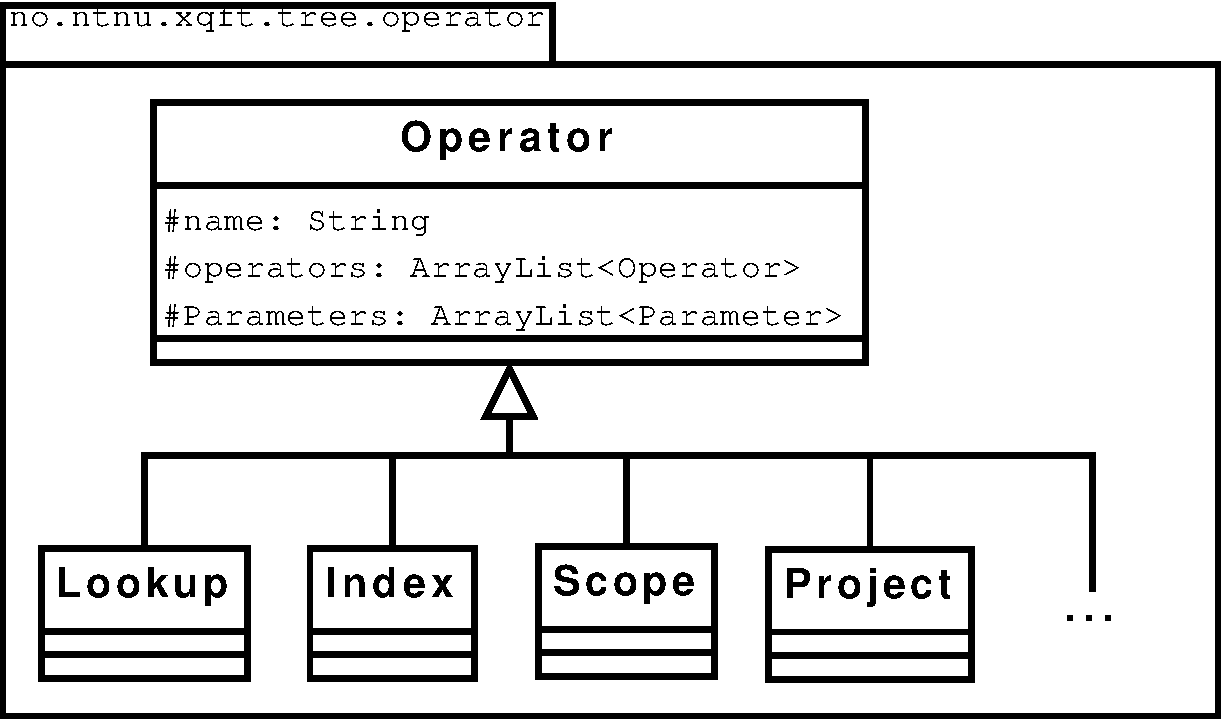
\includegraphics[scale=0.5]{diagrams/mql_operator_uml}
  \caption{Simplified class diagram of MQL operators}
  \label{fig:impl:mql_op_uml}
\end{center}
\end{figure}
The operators modeled in the implementation correspond to the operators
described in section \ref{sect:method:marsOperators}. A simplified class
diagram is shown in figure \ref{fig:impl:mql_op_uml}. Note that the
responsibility with regards to converting an operator to a string
representation is largely left to the various subclasses. However, the default
fallback for the \texttt{Operator} class is to return a string of the form
\begin{Verbatim}
operator_name(param1, param2, ..., paramN; 
              operator1, operator2, ..., operatorM)
\end{Verbatim}
This is sufficient in some cases, such as for the model of the \texttt{cross()}
operator.

\begin{figure}[!htp]
\begin{center}
  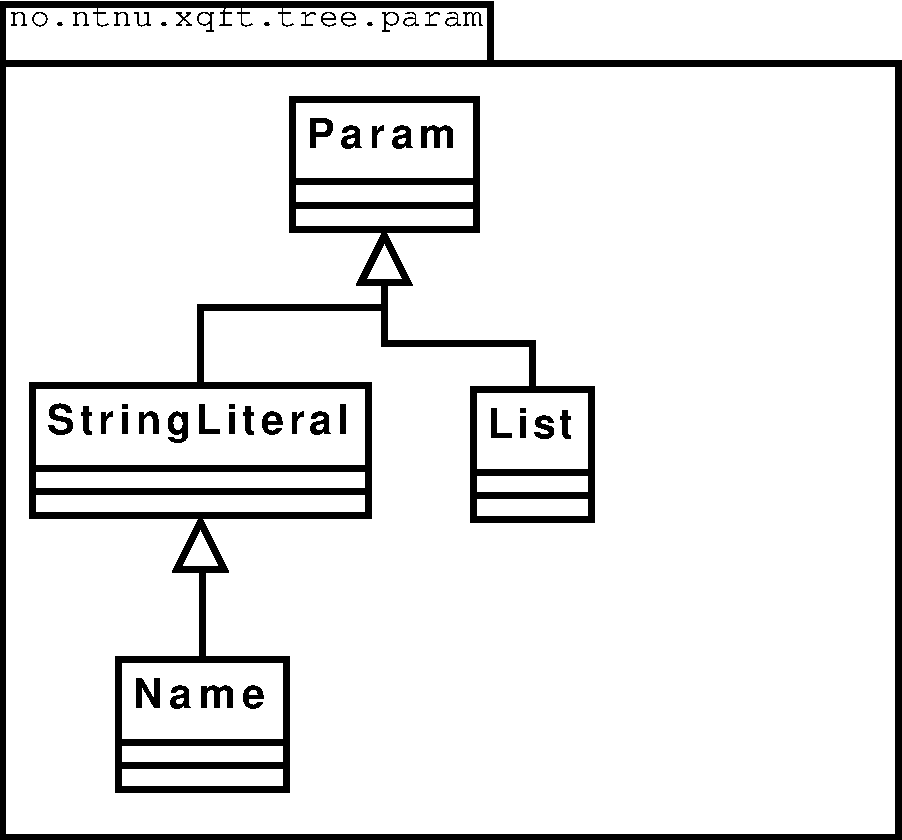
\includegraphics[scale=0.5]{diagrams/mql_param_uml}
  \caption{Class diagram of MQL parameters}
  \label{fig:impl:mql_param_uml}
\end{center}
\end{figure}

MQL parameters (as described in \ref{sect:method:mql:concepts}) are modeled as
seen in figure \ref{fig:impl:mql_param_uml}. Parameters require no complex
structure, and are only created and added to operators as needed.

\subsection{Concepts}
As mentioned, MQL queries are represented as trees, where each node represents
an operator. Each node is an instance of an operator class (as described
above), and contains a list of child operators and a list of parameters. To
convert the operator tree to a MQL query string, simply call the method
\texttt{toPrettyString(0)} on the root node of the operator tree.

\subsection{Usage}
The operator classes are designed to be intuitive and simple to use. Figure
\ref{fig:impl:mql_op_ex1_java} shows one example where a simple operator tree
is built and converted to an MQL query string (the result of which can be seen
in figure \ref{fig:impl:mql_op_ex1_mql}).

%\usepackage{graphics} is needed for \includegraphics
\begin{figure}[htp]
\begin{center}
  \begin{Verbatim}
Lookup lookup = new Lookup("Death in the clouds");
Scope scope = new Scope("/books/book/title", lookup);
Project project = new Project("author", scope);
System.out.println(project.toPrettyString(0));
  \end{Verbatim}
  \caption{Example java code to construct a MQL operator tree}
  \label{fig:impl:mql_op_ex1_java}
\end{center}
\end{figure}

\begin{figure}[htp]
\begin{center}
  \begin{Verbatim}
project([author];
  scope(/books/book/title;
    lookup("Death in the clouds")))
  \end{Verbatim}
  \caption{Resulting MQL query string from example in figure
  \ref{fig:impl:mql_op_ex1_java}}
  \label{fig:impl:mql_op_ex1_mql}
\end{center}
\end{figure}


\section{Context-sensitive visitor}
\subsection{Basics}
\subsection{Modifying the XQFTTree class}
\subsection{Rewrite visitor}
\subsection{Translation visitor}

\section{Scoping and symbol tables}
\begin{itemize}
  \item Holder styr p\aa~variabler, og om de er iterasjonsvariabler i n\aa v\ae
  rende scope
  \item Scope pushes rett f\oe r forclause, og poppes etter at returnclausen har
  blitt evaluert
  \item Symbolene er innkapslet i en symtabentry som inneholder metadata
\end{itemize}

\section{Passing metadata between nodes}
\subsection{Variable references}
\subsection{Singleton nodes}
\subsection{The TraverseReturn class}

\section{Tainting dependencies}
Dette blir den lengste seksjonen i dette kapittelet, h\aa per jeg.
\subsection{FLWOR expressions}
\subsection{Sequences}
\begin{itemize}
  \item behandler parantes istf. komma for sekvenser (ref spec) 
\end{itemize}

\section{Data flow}
\begin{itemize}
  \item grammatikk -> antlr -> parser
  \item xquery -> parser -> visitor -> relalg
\end{itemize}

\section{Visible external API}
\begin{itemize}
  \item Vise hvordan oversetteren kan brukes i sin helhet i andre programmer
\end{itemize}

\section{Command line interface}
Dette er ikke s\aa~veldig viktig \aa~skrive om, men greit \aa~ha med.
\begin{itemize}
  \item Argsengine
  \item Aksepterer flere strenger og filer
  \item Outputter til graphviz/dot og pdf, hvis tilgjengelig
  \item Dependencies (jar-filer og drit)
\end{itemize}

\section{Optimalisations?}

\section{Summary}
\label{sect:impl:summary}
\begin{itemize}
  \item sammendrag av dette kap
\end{itemize}